\documentclass[10pt, spanish]{beamer}
\usepackage[spanish]{babel}

\usetheme[progressbar=frametitle]{metropolis}

\usepackage{booktabs}
\usepackage[scale=2]{ccicons}

\usepackage{pgfplots}
\usepgfplotslibrary{dateplot}

\usepackage{float}
\graphicspath{ {images/} }

\usepackage{algpseudocode}
\usepackage{algorithm}
\usepackage{listings}

%% COLOR
\usepackage{color, colortbl}
\definecolor{Gray}{gray}{0.9}	
\definecolor{LightCyan}{rgb}{0.88,1,1}

\title{Identificaci\'on de patrones y algoritmos de consolidaci\'on en bases de datos de posicionamiento}
\date{\today}
\author{\textsc{Pilar Barbero Iriarte}\\
Director: \textit{Tom\'as Alcal\'a Nalv\'aiz}}
\institute{Universidad de Zaragoza}
\titlegraphic{\hfill
\includegraphics[height=1.5cm]{unizar.png}}

%%%%%%%%%%%%%%%%%%%%PYTHON CODING

% Default fixed font does not support bold face
\DeclareFixedFont{\ttb}{T1}{txtt}{bx}{n}{11} % for bold
\DeclareFixedFont{\ttm}{T1}{txtt}{m}{n}{11}  % for normal

% Custom colors
\usepackage{color}
\definecolor{deepblue}{rgb}{0,0,0.5}
\definecolor{deepred}{rgb}{0.6,0,0}
\definecolor{deepgreen}{rgb}{0,0.5,0}

% Python style for highlighting
\newcommand\pythonstyle{\lstset{
language=Python,
basicstyle=\ttm,
otherkeywords={self},             % Add keywords here
keywordstyle=\ttb\color{deepblue},
emph={MyClass,__init__},          % Custom highlighting
emphstyle=\ttb\color{deepred},    % Custom highlighting style
stringstyle=\color{deepgreen},
frame=tb,                         % Any extra options here
showstringspaces=false,           % 
basicstyle=\small,
columns=fullflexible,
}}


% Python environment
\lstnewenvironment{python}[1][]
{
\pythonstyle
\lstset{#1}
}
{}

% Python for external files
\newcommand\pythonexternal[2][]{{
\pythonstyle
\lstinputlisting[#1]{#2}}}

% Python for inline
\newcommand\pythoninline[1]{{\pythonstyle\lstinline!#1!}}
%%%%%%%%%%%%%%%%%%%%%%%%%%%%%%%%%

\begin{document}

\maketitle


%\section{Introducci\'on}

%%Introducci\'on
\begin{frame}[fragile]
\frametitle{Introducci\'on}
Contexto: 
\begin{itemize}
	\item Empresa Zaragozana de telecomunicaciones.
	\item Almacenamiento de posiciones GPS de sujetos.
	\item Capacidad de guardado de posiciones limitada.
\end{itemize}
\end{frame}


\begin{frame}[fragile]
\frametitle{Introducci\'on}
Problemas:
	\begin{itemize}
		\item Exceso de \'estas.
		\item No existe preprocesado antes de la inserci\'on.
		\item No existe postprocesado despu\'es de la inserci\'on.
		\item No todas aportan informaci\'on.
	\end{itemize}
\end{frame}

%%OBJETIVO
\begin{frame}[fragile]
  \frametitle{Introducci\'on}
  Objetivo:
  \begin{itemize}
  	  \item Eliminar posiciones repetidas.
  	  \item Eliminar posiciones que no aporten informaci\'on.
   \end{itemize}
\end{frame}

%\section{An\'alisis de los datos}


\begin{frame}[fragile]
\frametitle{An\'alisis de los datos}
  \begin{itemize}[<+- | alert@+>]    
\item \textbf{Id}: Identificador num\'erico
\item \textbf{IdServidor}: Identificador num\'erico del servidor que realiza la inserci\'on
\item \textbf{Recurso}: identificador del sujeto que transfiere la posici\'on
\item \textbf{Latitud}: real que representa la latitud GPS
\item \textbf{Longitud}: real que representa la longitud GPS
\item \textbf{Velocidad}: entero que representa la velocidad instant\'anea
\item \textbf{Orientaci}\'on: entero que representa la orientaci\'on respecto al norte en grados
\item \textbf{Cobertura}: booleano que indica si tiene cobertura (n. sat\'elites)
\item \textbf{Error}: error en la toma de posici\'on
  \end{itemize}
\end{frame}

%\section{¿C\'omo abordar el problema?}
\begin{frame}[fragile]
\frametitle{¿C\'omo abordar el problema?}
\begin{itemize}

\item Desarrollo de algoritmos de consolidaci\'on a trav\'es de nociones de distancia y tiempo.

\item Uso de algoritmos de \textit{clustering} con el fin de identificar varias posiciones con su centro del cl\'uster y consolidarlas en \'esta.

\end{itemize}
\end{frame}

%\section{Noci\'on de posici\'on y cl\'uster}

\begin{frame}[fragile]
\frametitle{Posici\'on}
Se define la clase \texttt{Position} en Python de la siguiente manera:\\
\bigskip
\begin{python}
class Position:
    def __init__(self, id, resource, lat, lon, speed, track, date):
        self.id = id
        self.resource = resource
        self.lat = lat
        self.lon = lon
        self.speed = speed
        self.track = track
        self.date = date
\end{python}
\end{frame}

\begin{frame}[fragile]
\frametitle{Cl\'uster}
Se define la clase de \texttt{Cl\'uster} en Python de la siguiente manera:\\
\bigskip
\begin{python}
class Cluster:
"Cluster of points"
    def __init__(self, center, points):
	self.center = center
	self.points = points
\end{python}

\end{frame}


%\section{M\'etodos simples}

\begin{frame}[fragile]
\frametitle{Nociones de vecindario}

Distintas nociones de vecindario para los algoritmos de consolidaci\'on simple,
\begin{itemize}
	\item Vecindario utilizando la distancia eucl\'idea
	\item Vecindario involucrando velocidad
	\item Vecindad $t_0-$alcanzable
	\item Vecindad involucrando el tiempo
\end{itemize}
\end{frame}

%%%%%%%%%%%%%%%%%%%%%%%%%%%%%%
\begin{frame}[fragile]
\frametitle{Vecindario utilizando la distancia eucl\'idea}

Utilizando la distancia eucl\'idea, definimos un vecindario de la siguiente manera:\\

$$ d_E(p_0, p) = \sqrt{(lat_{p} - lat_{p_0})^2 + (long_{p} - long_{p_0})^2 } < \varepsilon $$

donde $p$ es un punto con latitud $lat_{p}$ y longitud $long_{p}$.\\

\bigskip
\begin{python}
    def IsInNeighEUSimple(self, q, eps):
	return self.distance_eu(q) < eps
\end{python}

\end{frame}

%%%%%%%%%%%%%%%%%%%%%%%%%%%%%%

\begin{frame}[fragile]
\frametitle{Vecindario involucrando velocidad}

En el momento que se toma la posici\'on $p_0$, aparte de la latidud y su longitud, se toma la velocidad instant\'anea del sujeto.
A mayor velocidad, puntos m\'as alejados de lo que considerar\'iamos en el primer caso (fuera de nuestro vecindario simple), podr\'ian estar dentro de nuestro nuevo radio, que depender\'ia de la velocidad instant\'anea.

$$ d_E(p_0, p) = \sqrt{(lat_{p} - lat_{p_0})^2 + (long_{p} - long_{p_0})^2 } < \varepsilon \cdot vel_{p_0} $$

\bigskip
\begin{python}
    def IsInNeighSpeedRelative(self, q, eps):
	if self.speed != 0:
	    return self.distance_eu(q) < eps * self.speed	
	else:
	    return False
\end{python}

\end{frame}
%%%%%%%%%%%%%%%%%%%%%%%%%%%%%%
\begin{frame}[fragile]
\frametitle{Vecindad $t_0-$alcanzable}

Fijando un intervalo de tiempo $t_0$, se define una vecindad $t_0$-alcanzable como aquellos puntos que nuestro sujeto puede alcanzar en un tiempo $t_0$. Un sujeto que se desplace a velocidad reducida, tendr\'a una vecindad $t_0$-alcanzable m\'as reducida que otro que se desplace a una velocidad superior. Redefiniremos el radio de nuestro vecindario a trav\'es de la velocidad instant\'anea que lleve nuesto sujeto, es decir, $vel_{p_0}\cdot t_0$.  \\

$$ d_E(p_0, p) = \sqrt{(lat_{p} - lat_{p_0})^2 + (long_{p} - long_{p_0})^2 } < vel_{p_0} \cdot t_0 $$

\'Este es un caso concreto del vecindario involucrando la velocidad. \\

\bigskip
\begin{python}
    def IsInNeighT0Reachable(self, q, t0):
	return self.distance_eu(q) < t0 * self.speed
\end{python}

\end{frame}
%%%%%%%%%%%%%%%%%%%%%%%%%%%%%%

\begin{frame}[fragile]
\frametitle{Vecindad involucrando el tiempo}
Las posiciones de nuestros sujetos vienen muestreadas adem\'as con el instante en el que fueron tomadas. Podemos considerar que el tiempo entre tomas tambi\'en es una distancia y definir un vecindario. Definimos esta distancia temporal como la resta de ambos instantes, y el vecindario como: 

$$ d_T(p_0, p) = time_p - time_{p_0} < \delta $$

\bigskip

\begin{python}
    def is_neighboorhoudByTime(self, q, lapse):
	time1 = time.mktime(self.date.timetuple())
	time2 = time.mktime(q.date.timetuple())
	return abs(time1 - time2) < lapse
\end{python}

\end{frame}

\begin{frame}[fragile]
\frametitle{Consolidaci\'on por distancia}
Utilizando los tres tipos de vecindarios que hemos definido, definimos el
siguiente m\'etodo que realizará la consolidaci\'on del tipo que le indiquemos:\\

\bigskip

\begin{algorithmic}[1]
\Function{ConsolidationByDistance}{$positions, typeOfDistance, eps, t0$}
\For{\textbf{each} pos \textbf{in} positions}
        \If{$pos.IsInNeighBorhood(typeOfDistance, next(pos), eps)$}
        		\State{Remove position in DB}
        \Else
        		\State{Maintain position in DB}
        \EndIf
\EndFor
\EndFunction
\end{algorithmic}
\end{frame}


\begin{frame}[fragile]
\frametitle{Experimento utilizando consolidaci\'on por distancia}
Se fija un $\varepsilon = 0.0001$ y se realiza una consolidaci\'on utilizando la distancia eucl\'idea:\\

\bigskip

\begin{figure}[H]
	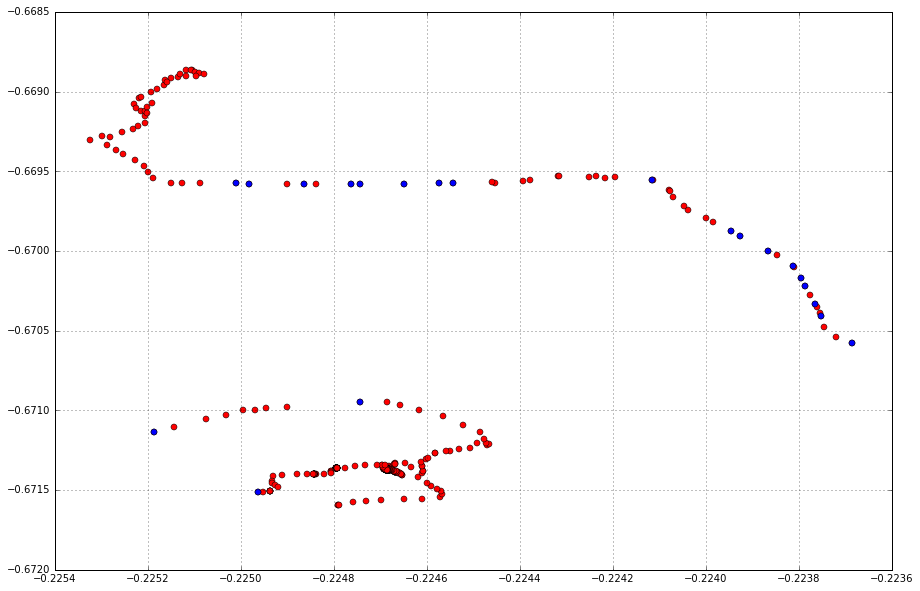
\includegraphics[scale=.25]{distanceEuEps10-4.png}
	\caption{Resultado consolidaci\'on por distancia Simple}
\end{figure}

\end{frame}

\begin{frame}[fragile]
\frametitle{Consolidaci\'on por tiempo}

Se fija un lapso de tiempo que se debe cumplir entre posici\'on y posici\'on, y se eliminan todas aquellas que est\'en cuya distancia temporal con su siguiente est\'e por debajo de este lapso fijado.\\

\bigskip
\begin{algorithmic}[1]
\Function{ConsolidationByTime}{$positions, lapse$}
	\For{\textbf{each} pos in positions}
		\State{$nextpos = pos++$}
		\If{$IsInNeighboorhodByTime(nextpos, pos, lapse)$}
			\State{Remove pos}
		\EndIf
	\EndFor
\EndFunction
\end{algorithmic}
\end{frame}


\begin{frame}[fragile]
\frametitle{Experimento utilizando consolidaci\'on por tiempo}
Se realiza una consolidaci\'on por tiempo con un lapso de 20 segundos:\\

\bigskip

\begin{figure}[H]
	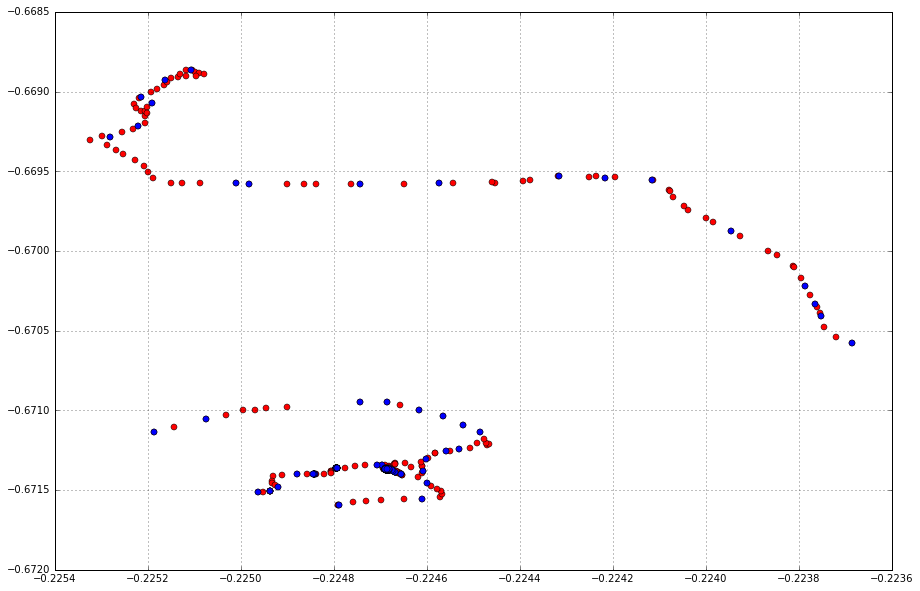
\includegraphics[scale=.25]{byTimeSuj1.png}
	\caption{Resultado consolidaci\'on por tiempo}
\end{figure}

\end{frame}


\begin{frame}[fragile]
\frametitle{Consolidaci\'on por adelgazamiento}
Se puede recurrir a un tipo de consolidaci\'on en la cual dada una lista de posiciones normalmente antiguas, se elimine un subconjunto de estas, por ejemplo, 3 de cada 5.\\
\bigskip
\begin{algorithmic}[1]
\Function{ConsolidationByThinning}{$positions, j, k$}\Comment{$j < k$}
	\For{\textbf{each} pos in positions}
		\If{$position.Index \% k == 0$}
			\For{$i = 0; i < k; i++$}
				\State{Remove position with index == position.Index}
			\EndFor
		\EndIf
	\EndFor
\EndFunction
\end{algorithmic}
\end{frame}


\begin{frame}[fragile]
\frametitle{Experimento utilizando consolidaci\'on por adelgazamiento}
Se realiza una consolidaci\'on por adelgazamiento, se mantienen 2 posiciones de cada 5:\\

\bigskip

\begin{figure}[H]
	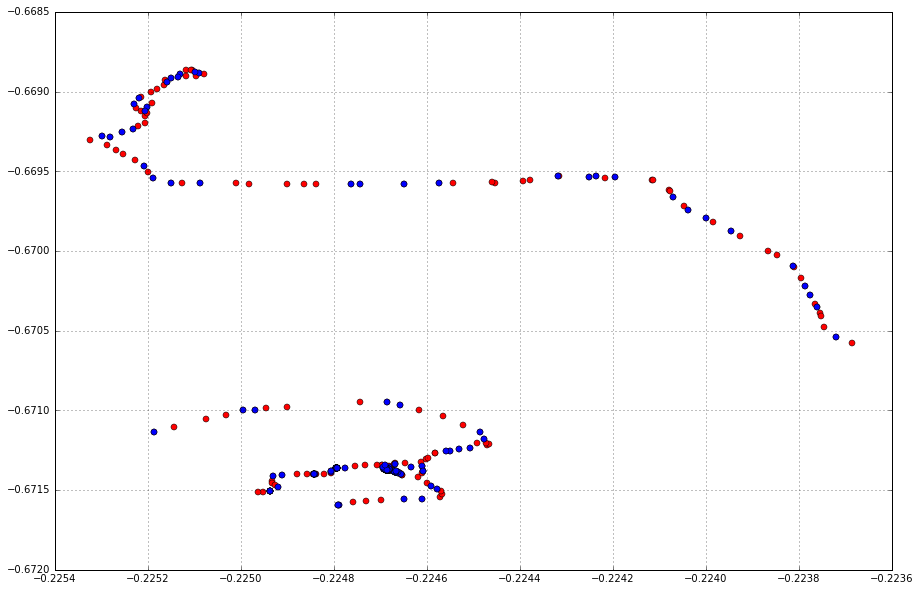
\includegraphics[scale=.25]{thinningSuj1.png}
	\caption{Resultado consolidaci\'on por adelgazamiento}
\end{figure}

\end{frame}



\begin{frame}[fragile]
\frametitle{M\'etodos avanzados}

\textbf{Algoritmos de consolidaci\'on asociados a m\'etodos de clustering}\\

\bigskip

Un an\'alisis cl\'uster es un conjunto de t\'ecnicas multivariantes utilizadas para clasificar a un conjunto de individuos en grupos homog\'eneos. Hemos elegido una serie de t\'ecnicas de aprendizaje no supervisado ya que \'este parte de que no hay un conocimiento a priori y es \'util en t\'ecnicas de compresi\'on de datos.


\begin{itemize}
\item \textbf{K-means}
\item \textbf{DBSCAN}
\item \textbf{DJ-Cl\'uster}
\end{itemize}

\end{frame}




\begin{frame}[fragile]
\frametitle{K-means}
\textbf{K-means} es un m\'etodo eficiente de \textit{clustering} que tiene como objetivo la partici\'on de un conjunto de $n$ elementos en $k$ grupos distintos. Datao un conjunto de $n$ elementos, se construye dicha partici\'on $S=\{S_1, S_2, \ldots, S_k\}$ con el fin de minimizar el t\'ermino del error cuadr\'atico:

$$ \sum_{i=1}^{n} \sum_{x\in S_i} \text{d}(x,m_i)$$

donde $m_i$ es el centro de cada cl\'uster $S_i$ y $\text{d}(x, m_i)$ es la distancia definida entre el punto $x$ y $m_i$.

\end{frame}

\begin{frame}[fragile]
\frametitle{K-means}
Se procede:
\begin{enumerate}
	\item Se prefija un n\'umero de cl\'usters.
	\item Se asigna cada punto a su cl\'uster de manera aleatoria.
	\item Se itera sobre cada punto, encuentra el centro de cl\'uster m\'as cercano y se lo asigna a dicho cl\'uster.
	\item Se calcula el error y se reitera hasta que este error se minimiza o estabiliza.
\end{enumerate}
\end{frame}

\begin{frame}[fragile]
\frametitle{Experimento con K-means}
Se utiliza el software \texttt{Weka} sobre un sujeto con $2000$ posiciones para una consolidaci\'on al $25\%$, es decir, a $500$.

\begin{figure}[H]
	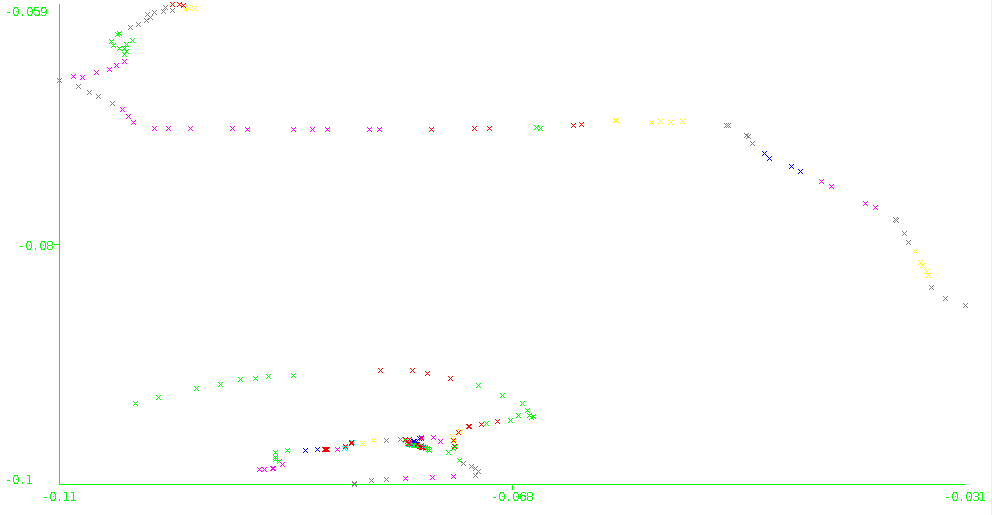
\includegraphics[scale=.35]{kMeansSujeto1.png}
	\caption{Resultado de \textbf{K-means}}
\end{figure}


\end{frame}

\begin{frame}[fragile]
\frametitle{Conclusiones K-means}

Resultados:
\begin{itemize}
\item 10 iteraciones 
\item Error cuadr\'atico: 0,117363
\item n\'umero de posiciones que ha agrupado por cl\'uster entre 1 y 9
\end{itemize}

\bigskip

Inconvenientes:
\begin{itemize}
	\item N\'umero de cl\'usters prefijado a 500.
	\item K-means no determin\'istico.
	\item No hay puntos considerados ruidos, s\'olo cl\'usters unipuntuales.
\end{itemize}
\end{frame}


%%%%%%%%%%%%%%%%%%%%%%%%%%%%%%%%%%%%%%%%%
%%%%%%%%%%%%%%%%%%%%%%%%%%%%%%%%%%%%%%%%%\\
%%%%%%%%%%%%%%%%%%%%%%%%%%%%%%%%%%%%%%%%%

\begin{frame}[fragile]
\frametitle{DBSCAN}
\textbf{DBSCAN}  es un algoritmo de clustering basado en la densidad por lo que encuentra el n\'umero de cl\'usters comenzando por una estimación de la distribución
de densidad de los nodos correspondientes. \\

\begin{itemize}
\item Punto $p$ n\'ucleo: si posee un n\'umero m\'inimo de puntos ($minPts$) en su vecindario sobre $\varepsilon$.
\item Punto alcanzable desde $p$: si existe un camino $p1=p, \ldots, p_n=q$ donde $p_{i+1}$ es alcanzable por $p_i$.
\item Aislados: puntos no considerados ni n\'ucleo ni alcanzables.

\smallskip
	\centering
	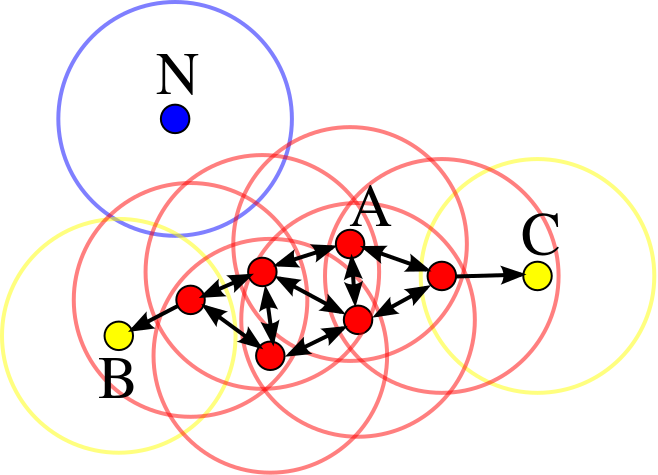
\includegraphics[scale=.2]{DBSCAN.png}
\end{itemize}
\end{frame}

\begin{frame}[fragile]
\frametitle{DBSCAN}
\textbf{DBSCAN} necesita de dos par\'ametros: $\varepsilon$ y $MinPts$.

\begin{algorithmic}[1]
\Function{DBSCAN}{$positions, eps, minPts$}
	\State{C = 0}
	\For{\textbf{each} pos in positions}
		\If{$pos$ has been visited}
			\State{Continue next position}
		\Else
			\State{Mark $pos$ as visited}
			\State{N(pos) = NeighborPts(pos, eps)}
			\If{$length(N(pos)) < MinPts$}
				\State{Mark $pos$ as noise}
			\Else
				\State{C = next Cluster}
				\State{expandCluster(pos, N(pos), C, eps, MinPts)}				
			\EndIf
		
		\EndIf
	\EndFor
\EndFunction
\end{algorithmic}
\end{frame}

\begin{frame}[fragile]
\frametitle{Experimento con DBSCAN}

Mismos datos que para \textbf{K-means}, sujeto con $2000$ posiciones. 

\begin{figure}[H]
	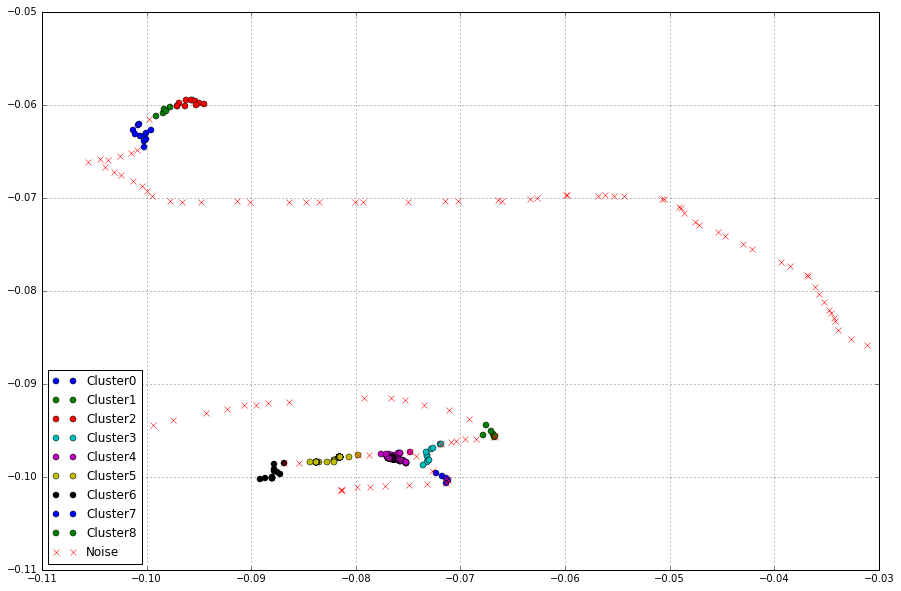
\includegraphics[scale=.3]{dbscanSujeto1.png}
	\caption{Resultado de \textbf{DBSCAN}}
\end{figure}

\end{frame}

%%%%%%%%%%%%%%%%%%%%%%%%%%%%%%%%%%%%%%%%%%%%%%%%%
%%%%%%%%%%%%%%%%%%%%%%%%%%%%%%%%%%%%%%%%%%%%%%%%%\\
%%%%%%%%%%%%%%%%%%%%%%%%%%%%%%%%%%%%%%%%%%%%%%%%%
%%%%%%%%%%%%%%%%%%%%%%%%%%%%%%%%%%%%%%%%%%%%%%%%%\\
%%%%%%%%%%%%%%%%%%%%%%%%%%%%%%%%%%%%%%%%%%%%%%%%%

\begin{frame}[fragile]
\frametitle{DJ-Cluster}
\textbf{Density-Joinable Cl\'uster} es un tipo de algoritmo de clustering basado en densidades de puntos.\\

\bigskip

\begin{algorithmic}[1]
	\For{\textbf{each} $p$ in set $S$}
		\State{Compute neighborhood $N(p)$ for $\varepsilon$ and $MinPts$}
		\If{$N(p)$ is null ($|N(p)| < MinPts$ for $\varepsilon$)}
			\State{Label $p$ as noise}
		\ElsIf{$N(p)$ is density-joinable to an existing cluster} 
			\State{Merge $N(p)$ with the cluster which is density-joinable}
		\Else
			\State{Create a new cluster $C$ based on $N(p)$}
		\EndIf
	\EndFor
\end{algorithmic}

\end{frame}

\begin{frame}[fragile]
\frametitle{Experimento con DJ-Cluster}
Utilizando \texttt{Weka} dado un $\varepsilon=0.0001$ y $minPts = 2$:\\

\begin{figure}[H]
	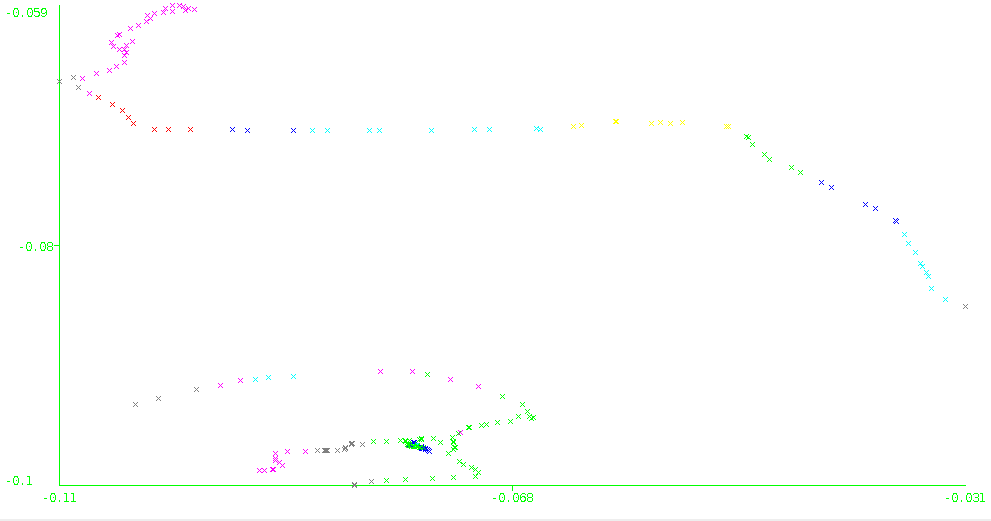
\includegraphics[scale=.43]{djClusterSujeto1.png}
	\caption{Resultado de \textbf{DJ-Cluster}}
\end{figure}

\end{frame}



%%%%%%%%%%%%%%%%%%%%%%%%%%%%%%%%%%%%%%%%%%%%%%%%%
%%%%%%%%%%%%%%%%%%%%%%%%%%%%%%%%%%%%%%%%%%%%%%%%%\\
%%%%%%%%%%%%%%%%%%%%%%%%%%%%%%%%%%%%%%%%%%%%%%%%%
%%%%%%%%%%%%%%%%%%%%%%%%%%%%%%%%%%%%%%%%%%%%%%%%%\\
%%%%%%%%%%%%%%%%%%%%%%%%%%%%%%%%%%%%%%%%%%%%%%%%%

\begin{frame}[fragile]
\frametitle{Comparativa t\'ecnicas simples}

\begin{center}
\begin{tabular}{|l|l|l|}
	\hline
	\rowcolor{Gray}
	M\'etodo & Tiempo & N. \\
	\hline	
	Cons. por adelgazamiento &  <0.01 sec & 800 \\
	\hline 
	Cons. por distancia simple &  <0.01 sec & 507 \\
	\hline
	Cons. por distancia $t_0-$alcanzable  &  <0.01 sec  & 21\\
	\hline
	Cons. por tiempo &  <0.01 sec  & 1786\\
	\hline
\end{tabular}
\end{center}

\begin{itemize}
	\item Alternar distintos tipos de consolidaci\'on en funci\'on del espacio cr\'itico en ese momento.
\end{itemize}
\end{frame}

%\section{Comparativa casos estudiados}
\begin{frame}[fragile]
\frametitle{Comparativa t\'ecnicas clustering}
\begin{center}
\begin{tabular}{|l|l|l|l|}
	\hline
	\rowcolor{Gray}
	M\'etodo & Tiempo & N. & Iteraciones\\
	\hline	
	K-means & 0.69 secs & 500 & 9\\
	\hline
	DBSCAN &  2 min 30 secs & 9 & 111 \\
	\hline
	DJ-Cluster &  0.37 secs & 22  & 11\\
	\hline
\end{tabular}
\end{center}

\begin{itemize}
	\item DBSCAN m\'as lento de todos.
	\item DBSCAN consolidaci\'on mayor.
	\item K-means se queda en 500 cl\'usters.
	\item DJ-Cl\'uster baja de los 500.
	\item DJ-Cl\'uster menor tiempo de ejecuci\'on.
\end{itemize}

\end{frame}



%\section{Conclusiones}
\begin{frame}[fragile]
\begin{itemize}[<+- | alert@+>]
	\item Algoritmos de consolidaci\'on simples son \textit{simples}, pero eficaces.
	\item Noci\'on de vecindario distinto al eucl\'ideo implementada en algoritmos de consolidaci\'on simple.
	\item Algoritmos de \textit{clustering} m\'as avanzados, pero m\'as complejos a la hora de implementar.
	\item Importante un procesado previo.
	\item A la hora de recuperar una traza con los datos borrados, mejor \textit{DJ-Cl\'uster}
	\item Noci\'on de ruido de DBSCAN importante, tanto DJ-Cl\'uster como K-means s\'olo encuentra cl\'usters de tama\~no 1.
\end{itemize}
\end{frame}

%\section{Demostraci\'on}

\begin{frame}[fragile]
\frametitle{Demo}
Demostraci\'on
\end{frame}

\begin{frame}[fragile]
	\frametitle{C\'odigo}
	\begin{center}
		\href{http://github.com/pbarbero/TFM}{http://github.com/pbarbero/TFM}
		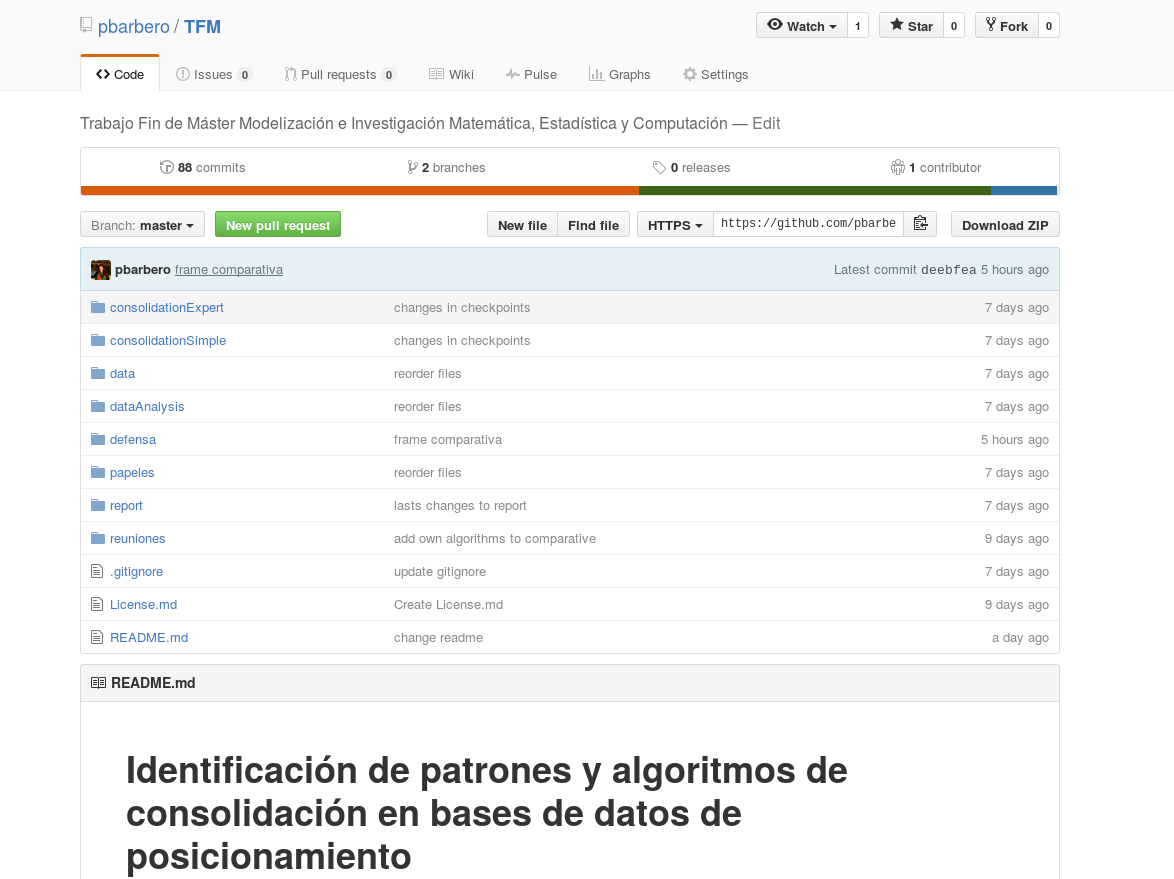
\includegraphics[scale=.3]{github.png}
	\end{center}
\end{frame}

\begin{frame}[fragile]
\frametitle{Preguntas}
Preguntas
\end{frame}

%\section{Preguntas}



\end{document}
